%
% komplex.tex -- Anhang über komplexe Zahlen
%
% (c) 2015 Prof Dr Andreas Mueller, Hochschule Rapperswil
%
\chapter{Komplexe Zahlen}
\lhead{Komplexe Zahlen}
\rhead{}
Der mathematische Formalismus der Quantenmechanik kann nicht ohne komplexe
Zahlen auskommen.
Leonhard Euler sah die Zahlen $\sqrt{-1}$ noch als imagin"ar an,
also als ohne Gegenst"uck in der realen Welt.
Elektroingenieure verwenden komplexe Zahlen mit grossem Erfolg in ihren
Anwendungen, sie spielen aber vor allem die Rolle eines praktischen
Werkzeugs. Die Regeln, mit denen am Schluss solcher Rechnungen sichergestellt
wird, dass die Resultate reell sind, zeigen ausserdem, dass man alles auch
ohne komplexe Zahlen durchrechnen k"onnte, wenn auch wesentlich weniger
elegant.

In der Quantenmechanik geht es aber nicht mehr ohne komplexe Zahlen,
die physikalischen Gr"ossen selbst sind komplex. Es gibt zwar auch
hier wieder Regeln, die sicherstellen, dass Messresultate reell sind
(Operatoren m"ussen selbstadjungiert sein), aber sie erlauben nicht,
die ganze Quantenmechanik auf eine Art zu beschreiben, die ohne komplexe
Zahlen auskommt.

\section{Der K"orper $\mathbb C$ der komplexen Zahlen}
\rhead{Der K"orper $\mathbb C$}
In den reellen Zahlen $\mathbb R$ k"onnen alle Grundoperationen ausgef"uhrt
werden, es ist jedoch nicht m"oglich, die Quadratwurzeln aus negativen
Zahlen zu ziehen. Eine analoge Situation trifft man schon viel fr"uher.
In den nat"urlichen Zahlen $\mathbb N$ kann man zwar addieren und
multiplizieren, aber nicht subtrahieren.
F"ugt man die negativen Zahlen hinzu erh"alt man eine Menge $\mathbb Z$,
in der die Subtraktion uneingeschr"ankt m"oglich ist. Division ist aber
immer noch nur f"ur spezielle Divisoren m"oglich. F"ugt man jedoch die
Br"uche zu $\mathbb Z$ hinzu, erh"alt man die Menge der rationalen Zahlen
$\mathbb Q$, in der Division uneingeschr"ankt m"oglich ist.
Doch auch $\mathbb Q$ ist nicht vollst"andig, die Zahl $\sqrt{2}$ ist
keine rationale Zahl. Nat"urlich kann man $\sqrt{2}$ durch eine
Folge von Br"uchen $r_n\in\mathbb Q$ approximieren, doch der Grenzwert
dieser Folge $\lim_{n\to\infty}r_n=\sqrt{2}$ ist nicht in $\mathbb Q$.
F"ugt man jedoch alle Grenzwerte von konvergenten Folgen zu $\mathbb Q$
hinzu, erh"alt man die Menge $\mathbb R$ der reellen Zahlen, in der
auch beliebige Wurzeln von positiven Zahlen gezogen werden k"onnen,
oder andere Grenzwerte wie $\pi$, $e$, die Werte von $\sin x$ und $\cos x$
und weitere.

\subsection{Grundoperationen f"ur die komplexen Zahlen}
Nach analogem Muster k"onnen wir auch $\mathbb R$ erweitern, so dass auch
die Wurzeln aus negativen Zahlen bestimmt werden k"onnen. Es reicht
sogar, nur die Wurzel von $-1$ hinzuzuf"ugen, denn jede andere Wurzel
einer negativen Zahl ist $\sqrt{-a}=\sqrt{-1}\cdot\sqrt{\mathstrut a}$.
Euler hat die Bezeichnung $i=\sqrt{-1}$ f"ur die imagin"are Einheit eingef"uhrt.
Es gilt nat"urlich $i^2=-1$.
\index{imaginare Einheit@imagin\"are Einheit}

\begin{definition}
Die Menge $\mathbb C=\{a+bi\,|\,a,b\in\mathbb R\}$ heisst die Menge der
\index{komplexe Zahl}%
\index{C@$\mathbb C$}%
{\em komplexen Zahlen}. Die komplexe Zahl $z=a+bi$ hat
Realteil $\operatorname{Re}z=a$ und Imagin"arteil $\operatorname{Im}z=b$.
\index{Realteil}%
\index{Imaginarteil@Imagin\"arteil}%
\index{komplexe Zahl!Realteil}%
\index{komplexe Zahl!Imagin\"arteil}%
Die Rechenoperationen sind so zu verstehen, dass die Rechenregeln
der Algebra erhalten bleiben\footnote{Man nennt dies das Permanenz-Prinzip}.
\end{definition}

Die Rechenoperationen folgen aus der Definition:
\begin{align*}
(a+bi)+(c+di)&=(a+c)+(b+d)i\\
(a+bi)(c+di)&=ac-i^2bd+(ad+bc)i=ac-bd+(ad+bc)i
\end{align*}
Die Division stellt noch ein Problem dar. Hier hilft das Konzept der
konjugiert komplexen Zahl.
\index{komplexe Zahl!Division}%

\begin{definition}
Die Zahl $\bar z=a-bi$ heisst die zu $z=a+bi$ {\em konjugiert komplexe} Zahl.
\end{definition}
\index{konjugiert komplex}

Zun"achst kann man mit der konjugiert komplexen Zahl den Betrag einer
komplexen Zahl definieren:
\[
z\bar z=(a+bi)(a-bi)=a^2+abi-abi-i^2b^2=a^2+b^2\qquad\Rightarrow\qquad
|z|^2=z\bar z.
\]
Andererseits kann man damit auch komplexe Br"uche berechnen, indem man
mit der konjugiert komplexen Zahl des Nenners erweitert:
\begin{align*}
\frac{a+bi}{c+di}&=
\frac{a+bi}{c+di}
\cdot
\frac{c-di}{c-di}=\frac{ac+bd+(bc-ad)i}{c^2+d^2}
\end{align*}
Die komplexen Zahlen k"onnen in einer Ebene visualisert werden: 
Realteil und Imagin"arteil werden entlang orthogonaler Achsen abgetragen.
Die Punkte $(x,y)$ der $x$-$y$-Ebene entsprechen also der komplexen Zahl
$x+yi$ der komplexen Zahlenebene (Abbildung~\ref{skript:gaussebene}).
\begin{figure}
\centering
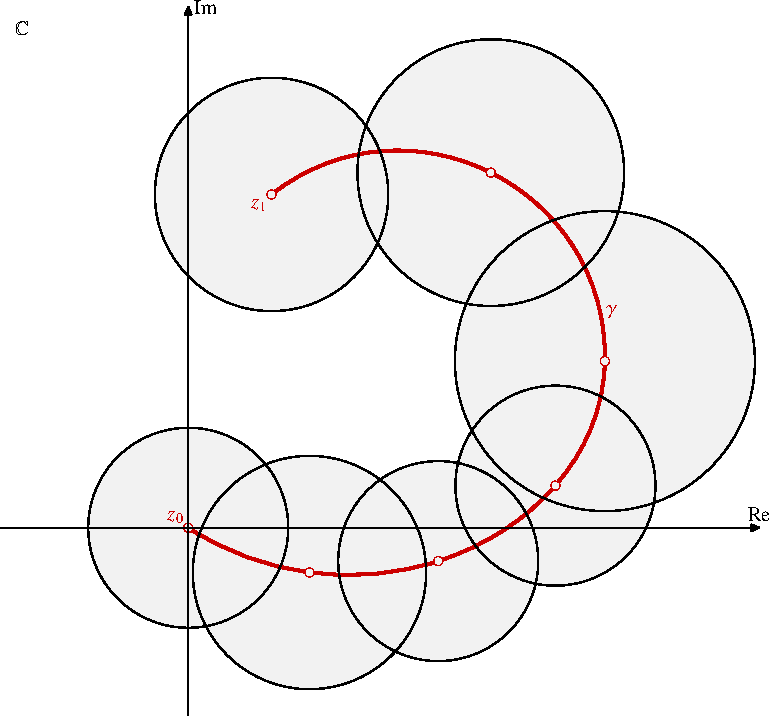
\includegraphics{graphics/komplex-1.pdf}
\caption{Komplexe Zahlenebene
\label{skript:gaussebene}}
\end{figure}
\index{Gauss-Ebene}%
\index{komplexe Zahlenebene}%

Mit Hilfe der komplexen Konjugation kann man den Real- and Imagin"arteil
einer komplexen Zahl $z=a+bi$ direkt ausdr"ucken:
\begin{align}
\operatorname{Re}z 
&=
a=\frac{(a+bi)+(a-bi)}2=\frac{z+\bar z}2
\label{skript:realteil-formel}
\\
\operatorname{Im}z
&=
b=\frac{(a+bi)-(a-bi)}{2i}=\frac{z-\bar z}{2i}.
\label{skript:imaginaerteil-formel}
\end{align}

\subsection{Polardarstellung}
\index{komplexe Zahl!Polardarstellung}
Die Darstellung der komplexen Zahlen als Punkte einer Ebene suggeriert
auch eine alternative Schreibweise.
Ein Punkt $z$ der komplexen Ebene kann auch charakterisiert werden mit Hilfe von
Polarkoordinaten, also durch seine Entfernung $r=|z|$ vom Nullpunkt,
und durch Polarwinkel zwischen der reellen Achse und der Richtung
zur komplexen Zahl. Der Polarwinkel heisst auch {\em Argument} $\operatorname{arg}z$,
\index{Argument}%
und es gilt
\[
\tan\operatorname{arg}z=\frac{\operatorname{Im}z}{\operatorname{Re}z}.
\]
\index{komplexe Zahl!Argument}
\index{komplexe Zahl!Betrag}
\index{komplexe Zahl!Multiplikation}
Die Multiplikation von komplexen Zahlen bekommt in der Polardarstellung
eine besondere Interpretation:
\begin{align*}
z_1z_2
&=
(r_1\cos\varphi_1+ir_1\sin\varphi_1) (r_2\cos\varphi_2+ir_2\sin\varphi_2)
\\
&=
r_1r_2(\cos\varphi_1+i\sin\varphi_1) (\cos\varphi_2+i\sin\varphi_2)
\\
&=
r_1r_2\bigl(
\cos\varphi_1\cos\varphi_2-\sin\varphi_1\sin\varphi_2 +
(\cos\varphi_1\sin\varphi_2+\sin\varphi_1\cos\varphi_2)i\bigr)
\\
&=
r_1r_2(\cos(\varphi_1+\varphi_2)+i\sin(\varphi_1+\varphi_2))
\\
\Rightarrow \operatorname{arg}z_1z_2&=\arg z_1 + \arg z_2
\end{align*}
Die Multiplikation zweier komplexen Zahlen entspricht also der
Multiplikation der Betr"age, und der Addition der Argumente.

Wir versuchen jetzt, die Werte der Exponentialfunktion zu $e^z$ zu
bestimmen.
Die Exponentialgesetze sollten auch weiterhin gelten.
Sei also $z=a+bi$, dann ist
\[
e^z=e^{a+bi}=e^a\cdot e^{bi}.
\]
Die Exponentialfunktion reeller Zahlen ist bereits wohlbekannt, es muss
also nur noch untersucht werden, welche Bedeutung $e^{bi}$ hat.

Betrachten wir die Funktion $f(t)= e^{it}$. Die Ableitungen von $f$ sind
\begin{align}
f'(t)&=ie^{it}=if(t)\notag\\
f''(t)&=-f(t).\label{skript:exp-dgl}
\end{align}
Die Funktion $f$ muss also eine L"osung der Differentialgleichung
(\ref{skript:exp-dgl}) sein, welche die Anfangsbedingungen $f(0)=1$ und
$f'(0)=if(0)=i$ erf"ullen muss.
Doch die Differentialgleichung (\ref{skript:exp-dgl}) hat die L"osungen
\[
f(t)=a\cos t+b\sin t.
\]
Setzt man die Anfangsbedingungen ein, findet man
\begin{align*}
f(0)&=1&\Rightarrow&&a&=1\\
f'(0)&=1&\Rightarrow&&b&=i,
\end{align*}
so dass wir jetzt $e^{it}$ ausrechnen k"onnen:
\begin{satz}[Euler]
\begin{align}
e^{it}=\cos t+i\sin t.
\label{skript:euler-formula}
\end{align}
\end{satz}
\index{Euler-Formel}%

Die komplexe Konjugation kehrt das Vorzeichen des Imagin"arteils um, also 
von $\sin t$. Da $\sin t$ eine ungerade Funktion ist, ist dies gleichbedeuten
damit, das Vorzeichen von $t$ zu kehren: $\overline{e^{it}}=e^{-it}$.

Mit der Eulerschen Formel sind wir jetzt auch in der Lage, den Zusammenhang
zwischen einer komplexen Zahl und ihrem Betrag und Argument sehr pr"agnant
auszudr"ucken:
\[
z=|r|\cdot e^{i\operatorname{arg}z}.
\]
Die Real- und Imagin"arteile von $e^{it}$ sind $\cos t$ und $\sin t$,
wir k"onnen sie auch mit den Formeln (\ref{skript:realteil-formel}) und
(\ref{skript:imaginaerteil-formel}) ausdr"ucken:
\begin{align*}
\cos t
&=
\operatorname{Re}e^{it}
=
\frac{e^{it}+\overline{e^{it}}}2
=
\frac{e^{it}+e^{-it}}2
\\
\sin t
&=
\operatorname{Im}e^{it}=\frac{e^{it}-e^{-it}}{2i}.
\end{align*}

\subsection{Matrixdarstellung der komplexen Zahlen\label{subsection:matrixdarstellung}}
\index{komplexe Zahl!Matrixdarstellung}
Die Algebra der komplexen Zahlen kann man auch als eine Algebra von Matrizen
schreiben. Dazu betrachten wir die Abbildung
\[
\varphi\colon
\mathbb C\to M_2(\mathbb R):
a+bi\mapsto\begin{pmatrix}a&b\\-b&a\end{pmatrix}
\]
Die imagin"are Einheit $i$ wird von $\varphi$ auf die Matrix
\[
\varphi(i)=J=\begin{pmatrix}0&1\\-1&0\end{pmatrix}
\]
abgebildet. Man kann nachrechnen, dass $J^2=-E$, und dass die Rechenregeln
f"ur die komplexen Zahlen durch die Abbildung $\varphi$ in die Rechenregeln
f"ur Matrizen transformiert werden.
Wir illustrieren dies f"ur die Multiplikation:
\[
\begin{aligned}
&(a+bi)(c+di)&&\mapsto&
&\begin{pmatrix}a&b\\-b&a\end{pmatrix}
\begin{pmatrix}c&d\\-d&c\end{pmatrix}
\\
&(ac-bd) + i(ad-bc)&&\mapsto&
&=\begin{pmatrix}
ac-bd&ad-bc\\
-ad+bc&ac-bd
\end{pmatrix}
\end{aligned}
\]
In dieser Darstellung kann man auch $e^{Jt}$ ausrechnen, indem man $Jt$ in
die Taylorreihe von $e^x$ einsetzt
\begin{align}
e^{Jt}
&=
E + tJ + \frac{t^2}{2!} J^2 + \frac{t^3}{3!} J^3 + \frac{t^4}{4!} J^4
 + \frac{t^5}{5!} J^5 + \frac{t^6}{6!} J^6 + \frac{t^7}{7!} J^7 + \dots
\notag
\\
&=
E + tJ - \frac{t^2}{2!} E - \frac{t^3}{3!} J + \frac{t^4}{4!} E
 - \frac{t^5}{5!} J - \frac{t^6}{6!} E + \frac{t^7}{7!} J + \dots
\notag
\\
&=\biggl(1 - \frac{t^2}{2!} + \frac{t^4}{4!} - \frac{t^6}{6!} + \dots\biggr) E
+ \biggl(t - \frac{t^3}{3!} + \frac{t^5}{5!} - \frac{t^7}{7!} + \dots\biggr) J
= E \cos t + J \sin t.
\label{skript:eulermatrixdarstellung}
\end{align}
Die Eulerformel (\ref{skript:euler-formula}) l"asst sich also auch in der
Matrixdarstellung der komplexen Zahlen wiedergewinnen.

\section{Komplexe Matrizen}
\rhead{Komplexe Matrizen}
\index{Matrix!komplex}%
Die Lineare Algebra im Bachelor wird typischerweise nur in den
reellen Zahlen entwickelt, der einzige untersuchte Vektorraum ist
der Raum $\mathbb R^n$ der reellen $n$-dimensionalen Vektoren.
F"ur die Quantenmechanik ben"otigen wir aber auch Vektoren mit
komplexen Komponenten. Der $n$-dimensionale komplese Vektorraum
$\mathbb C^n$ ist die Menge
\[
\left\{\left.\begin{pmatrix}c_1\\\vdots\\c_n\end{pmatrix}\,\right|
c_i\in\mathbb C\right\},
\]
mit der komponentenweisen Addition und der Multiplikation mit einer
komplexen Zahl. Nichts an der elementaren linearen Algebra hat besondere
Eigenschaften der reellen Zahlen verwendet, die nicht auch die komplexen
Zahlen haben. Der Gauss-Algorithmus, die Konstruktion der Determinanten,
ja sogar der grundlegende Algorithmus zur L"osung des Eigenwertprobems
funktioniert genau gleich auch f"ur komplexe Matrizen. Nur im Bereich
des Skalarproduktes sind minimale Modifikationen notwendig.

\subsection{Skalarprodukt f"ur komplexe Vektorr"aume}
In der linearen Algebra im ersten Semester wird das Skalarprodukt
geometrisch mit Hilfe der Projektion eingef"uhrt.
Eine solche Konstruktion ist f"ur komplexe Vektoren nicht m"oglich,
weil es keine anschauliche komplexe Geometrie gibt.

\subsubsection{Komplexes Skalarprodukt}
Um ein komplexes Skalarprodukt zu bekommen, gehen wir daher von den
algebraischen Eingeschaften des Skalarproduktes aus:
\begin{compactenum}
\item Das Skalarprodukt $(u,v)$ von komplexen Vektoren $u$ und $v$ ist linear
in $v$.
\item $(u,u) > 0$ falls $u\ne 0$.
\item Falls $(u,v)\in\mathbb R$, dann ist $(u,v)=(v,u)$.
\end{compactenum}
Diese Eigenschaften m"ussen auch f"ur ein komplexes Skalarprodukt gelten.
Wir zeigen, dass diese Eigenschaften auch ein komplexes Skalarprodukt 
weitgehend festlegt.

Zun"achst stellen wir fest, dass wir nicht erwarten k"onnen, dass
ein Skalarprodukt linear sein kann.
Betrachten wir dazu einen eindimensionalen Vektorraum $\mathbb C^1$.
Vektoren sind hier nur komplexe Zahlen, und ein Produkt, welches
linear in beiden Faktoren ist, ist von der Form $(u,v)=uv$. Dann ist
aber $(u,u)=u^2$, aber $u^2$ kann auch negativ sein, zum Beispiel f"ur $u=i$.
Das einzige Produkt, welches immer positiv ist, ist $(u,v)=\bar uv$.
Dieses Produkt ist aber nicht linear im Faktor $u$:
\[
(\lambda u,v)=\overline{(\lambda u)}v=\bar\lambda (\bar uv)=\bar\lambda (u,v).
\]
Wir m"ussen also von einem komplexen Skalarprodukt verlangen, dass es
\index{konjugiert linear}
im ersten Faktor {\em konjugiert linear} ist:
\[
(\lambda u,v)=\bar\lambda(u,v)
\]
Eine Funktion von zwei Vektoren, welche linear im zweiten Vektor ist
und konjugiert linear im ersten heisst {\em sesquilinear}.
\index{sesquilinear}%
\index{Sesquilinearform}%

Sei jetzt also $(\,\cdot\,|\,\cdot\,)$ eine Sesquilinearform.
Wir setzen $\lambda = 1/(u,v)$, dann gilt
$(u,\lambda v)$ reell ist. Dann gilt
\begin{align*}
1&=\lambda (u,v)=(u,\lambda v)=(\lambda v,u)=\bar\lambda(v,u)
&
&\Rightarrow&
\frac1{(\bar\lambda)}&=(v,u)
&
&\Rightarrow&
\overline{(u,v)}&=(v,u).
\end{align*}
Vertauschung der Faktoren ist also gleichbedeutend mit komplexer Konjugation
des Wertes des Skalarproduktes. Man nennt eine Funktion von zwei komplexen
Vektoren {\em hermitesch}, wenn $(u,v)=\overline{(v,u)}$ gilt.
\index{hermitesch}
\index{Matrix!hermitesch}

Eine hermitesche Sesquilinearform heisst {\em positiv definit}, wenn
\index{positiv definit}
f"ur jeden Vektor $u\ne 0$ gilt $(u,u)>0$. Diese Eigenschaft stellt
sicher, dass $(u,u)$ sinnvoll als die ``L"ange'' eines Vektors interpretiert
werden kann.

\begin{definition}
Ein komplexes Skalarprodukt ist eine positiv definite,
hermitesche Sesquilinearform.
\end{definition}
\index{Skalarprodukt!komplexes}

Das einfachste Beispiel eines komplexen Skalarproduktes ist
\[
(u,v)=\sum_i \bar u_iv_i.
\]
Die Standardbasisvektoren sind auch in diesem Skalarprodukt
orthonormiert.

%
% Adjungierte Matrix
%
\subsubsection{Adjungierte Matrix}
\index{adjungiert}
\index{Matrix!adjungiert}
\index{Abbildung!linear}
In den reellen Vektorr"aumen konnte man zu einer linearen $A$ immer
eine lineare Abbildung $A^t$ finden mit der Eigenschaft
$(u,Av)=(A^tu,v)$. Mit Hilfe der Standardbasisvektoren konnte
man auch ausrechnen, was dies f"ur die Matrizen von $A$ bedeutet:
\[
(e_i,A^te_j),
=
(A^te_j, e_i)
=
(e_j,Ae_i)=a_{ji}
\]
d.~h.~die Matrix von $A^t$ ist die transponierte Matrix von $A$.
Eine symmetrische Matrix war eine, die sich beim Transponieren nicht
"andert, also $A^t=A$.

Dasselbe kann man jetzt auch f"ur ein komplexes Skalarprodukt
versuchen. Zu einer komplexen Matrix $A$ ist also eine neue
Matrix $A^*$ gesucht, mit der Eigenschaft, $(A^*u,v)=(u,Av)$ f"ur 
jedes Paar von Vektoren $u$ und $v$. F"ur die Standardbasisvektoren
gilt dann
\[
(e_i,A^*e_j),
=
\overline{(A^*e_j, e_i)}
=
\overline{(e_j,Ae_i)}=\overline{a_{ji}},
\]
die Matrix von $A^*$ ist also nicht nur transponiert, sondern auch komplex
konjugiert. Hat $A$ die Ma\-trix\-e\-le\-men\-te $a_{ij}$ dann nennt man
die Matrix $A^*$ mit den Matrixelementen $\bar a_{ji}$ die
adjungierte Matrix. Eine Matrix, die sich beim Adjungieren nicht
"andert, heisst {\em selbstadjungiert}.
\index{Matrix!selbstadjungiert}
\index{selbstadjungiert}

Die Rechenregeln f"ur die adjungierte Matrix sind ganz "ahnlich wie
f"ur die Transposition:
\index{Transposition}%
\[
\begin{aligned}
(\lambda A)^*&=\bar\lambda A^*,
&
(A+B)^*&=A^*+B^*,
&
(AB)^*=B^*A^*.
\end{aligned}
\]
Man beachte, dass $A\mapsto A^*$ nicht linear ist.

\subsubsection{Unit"are Matrizen}
\index{unitar@unit\"ar}
Matrizen, die in reellen Vektorr"aumen das Skalarprodukt nicht "andern,
heissen orthogonal. Sie sind charakterisiert durch die Eigenschaft
\index{Matrix!orthogonal}%
\index{orthogonal}%
$(Ox,Oy)=(x,y)$, woraus sich mit Hilfe der Transposition ergibt:
\[
(Ox,Oy)=(O^tOx,y)=(x,y)\qquad\Rightarrow\qquad O^tO=E,
\]
woraus man weiter ablesen kann, dass bei orthogonalen Matrizen
die transponierte Matrix mit der invertierten Matrix zusammenf"allt.

F"ur komplexen Vekoren kann man wieder nach den Matrizen fragen, die das
komplexe Skalarprodukt nicht ver"andern. Eine Matrix $U$ hat diese
Eigenschaft, wenn
\[
(Ux,Uv)=(U^*Ux,y)=(x,y)\;\forall x,y
\qquad\Rightarrow\qquad
U^*U=E
\]
gilt,
eine solche Matrix heisst {\em unit"ar}. 
\index{unitar@unit\"ar}
\index{Matrix!unit\"ar}

F"ur reelle Matrizen $A$ ist $A^t=A^*$, also sind orthogonale Matrizen
auch unit"ar.

\begin{beispiel}
Die unit"aren $1\times 1$-Matrizen sind komplexe Zahlen $z$, welche
die zus"atzliche Bedingung $\bar zz=1$ erf"ullen m"ussen.
Die Menge der unit"aren $1\times 1$-Matrizen ist also
\[
U(1)=\left\{ z\in\mathbb C\,|\, |z|=1
\right\}.
\]
In der Quantenmechanik k"onnen Zustandsvektoren in der Regel nur bis auf
einen komplexen Faktor vom Betrag $1$, also bis auf ein Element
von $U(1)$ festgelegt werden.
Man spricht oft von ``bedeutungslosen'' Phasenfaktoren.
\end{beispiel}

\subsubsection{Die spezielle unit"are Gruppe $\operatorname{SU}(2)$}
\index{spezielle unit\"are Gruppe}
\index{SU(2)}
Wir betrachten Matrizen der Form
\begin{equation}
U=
\begin{pmatrix}
a&b\\-\bar b&\bar a
\end{pmatrix}
\label{skript:su2form}
\end{equation}
mit der zus"atzlichen Bedingung $|a|^2 + |b|^2=1$. Sie erf"ullen
\begin{align*}
U^*U
&=
\begin{pmatrix}
\bar a&-b\\\bar b&a
\end{pmatrix}
\begin{pmatrix}
a&b\\-\bar b&\bar a
\end{pmatrix}
=
\begin{pmatrix}
\bar aa+b\bar b & \bar ab-b\bar a\\
\bar ba-a\bar b & \bar bb+a\bar a
\end{pmatrix}
=
E
\\
\det(U)&=\left|
\begin{matrix}
a&b\\-\bar b&\bar a
\end{matrix}
\right|
=
a\bar a+\bar bb = |a|^2 + |b|^2=1.
\end{align*}
Solche Matrizen sind also nicht nur unit"ar, sondern haben auch Determinante 1.
Multipliziert man zwei Matrizen der Form (\ref{skript:su2form}),
wird das Produkt auch wieder Determinante 1 haben, aber es ist nicht klar,
dass es sich in der Form (\ref{skript:su2form}) schreiben l"asst.
Daher rechnen wir das Produkt aus, wir erhalten
\begin{align*}
\begin{pmatrix}  a                        & b                      \\
                 -\bar b                  & \bar a                 \end{pmatrix}
\begin{pmatrix}  c                        & d                      \\
                 -\bar d                  & \bar c                 \end{pmatrix}
&=
\begin{pmatrix}  ac-b\bar d               & ab+b\bar c             \\
                 -\bar bc-\bar a\bar d    & -\bar bd +\bar a\bar c \end{pmatrix}
=
\begin{pmatrix}  ac-b\bar d               & ab+b\bar c             \\
                 -(\overline{ab+b\bar c}) & \overline{ac-b\bar d}  \end{pmatrix}
.
\end{align*}
Das Produkt zweier Matrizen der Form (\ref{skript:su2form}) ist also wieder eine
Matrix der Form (\ref{skript:su2form}).
Die Menge dieser Matrizen ist demzufolge abgeschlossen unter
Matrixmultiplikation und Bildung der Inversen.
Man nennt diese Matrizen die Gruppe der speziellen unit"aren Matrizen:
\[
\operatorname{SU}(2)=\left\{
\left.
\begin{pmatrix}
a&b\\-\bar b&\bar a
\end{pmatrix}
\,
\right|
\,
a,b\in\mathbb C\wedge
|a|^2+|b|^2=1
\right\}.
\]
Die Gruppe $\operatorname{SU}(2)$ spielt bei der Analyse des Elektronenspins
eine wichtige Rolle.

Die Gruppe $\operatorname{SU}(2)$ ist eine Teilmenge der Menge der komplexen
$2\times 2$-Matrizen:
\[
\operatorname{SU}(2)
\subset
V=
\left\{
\left.
\begin{pmatrix}a&b\\-\bar b&\bar a\end{pmatrix}\,
\right|
a,b\in\mathbb C^2
\right\}
\subset
M_2(\mathbb C)
=\left\{
\left.
\begin{pmatrix}
a&b\\c&d
\end{pmatrix}
\,
\right|
\, a,b,c,d\in\mathbb C
\right\}
\]
Wir untersuchen die Menge $V$ etwas genauer.
Zun"achst k"onnen wir $V$ als zweidimensionalen komplexen Vektorraum
betrachten wie $\mathbb C^2$.
Als reeller Vektorraum betrachtet ist $V$ ein vierdimensionaler
reeller Vektorraum. Die Abbildung
\[
\mathbb R^4\to\mathbb C^2\to V
:
\begin{pmatrix}x_1\\x_2\\x_3\\x_4\end{pmatrix}\mapsto
\begin{pmatrix}x_1+ix_2\\x_3+ix_4\end{pmatrix}\mapsto
\begin{pmatrix} x_1+ix_2 & x_3+ix_4 \\
               -x_3+ix_4 & x_1-ix_2 \end{pmatrix}
\]
ist eine Bijektion zwischen $\mathbb R^4$, $\mathbb C^2$ und $V$.
Auch geometrisch ist $\mathbb C^2=\mathbb C\times \mathbb C$ das Produkt
von zwei Ebenen, hat also eine vierdimensionale Geometrie.
Darin ist $\operatorname{SU}(2)$ die Teilmenge der vierdimensionalen Vektoren,
und zwar derjenigen f"ur die gilt
\[
1
=
|a|^2+|b|^2
= 
x_1^2 + x_2^2 + x_3^2 + x_4^2,
\]
das sind die Vektoren von $\mathbb R^4$ mit L"ange $1$.
Geometrisch ist $\operatorname{SU}(2)$ also eine dreidimensionale Kugel
eingebettet in in einen vierdimensionalen Raum.

\subsubsection{Spur und Determinante}
Spur und Determinate k"onnen samt all ihren Rechenregeln sofort auf
komplexe Matrizen "ubertragen werden.
F"ur den Adjunktionsoperator finden wir die Rechenregeln
\[
\begin{aligned}
\det A^*&= \overline{\det A^t}=\overline{\det A},
&&\text{und}&
\operatorname{tr} A^*&=\overline{\operatorname{tr}A}.
\end{aligned}
\]
F"ur selbstadjungierte Matrizen kann man schliessen, dass sowohl
die Determinante wie auch die Spur von $A$ reell sein m"ussen.

In den komplexen Zahlen hat jedes Polynom $n$-ten Grades $n$ Nullstellen.
Daher k"onnen wir das charakteristische Polynom immer ausschreiben als
\begin{align*}
\det(A-\lambda E)
&=
(-1)^n (\lambda-\lambda_1)\dots(\lambda-\lambda_n)
\\
&=
(-1)^n(\lambda^n -(\lambda_1+\dots+\lambda_n)\lambda^{n-1}+\dots
+(-1)^n\lambda_1\dots\lambda_n
\\
&=
(-1)^n(\lambda^n - \operatorname{tr}A\lambda^{n-1}+\dots + (-1)^n\det A)
\end{align*}
Daraus k"onnen wir auch eine Formel f"ur $\det(E+tA)$ ableiten:
\begin{align}
\det(E+tA)
&=
(-t)^n\det\biggl(A-\frac1tE\biggr)
=
t^n\biggl(
\frac1{t^n}+\frac1{t^{n-1}}\operatorname{tr}A+\dots+\det A
\biggr)
\notag
\\
&=
1+t\operatorname{tr}A+\dots+t^n\operatorname{det}A
\label{skript:detandtrace}
\end{align}

%
% Eigenwertproblem fuer komplexe Matrizen
%
\subsection{Eigenwertproblem f"ur komplexe Matrizen}
\subsubsection{Definition}
Ein Vektor $v\ne 0$ heisst {\em Eigenvektor zum Eigenwert} $\lambda$ einer
\index{Eigenwert}
\index{Eigenvektor}
Matrix $A$, wenn $Av=\lambda v$ gilt. Diese Definition ist auch f"ur
komplexe Matrizen g"ultig, ebenso funktioniert der Standardalgorithmus
f"ur die L"osung des Eigenwertproblems nach wie vor:
\begin{enumerate}
\item Finde die Nullstellen der charakteristischen Gleichung
$\det(A-\lambda E)=0$.
\item F"ur jede Nullstelle $\lambda_i$, finde Eigenvektoren
durch L"osung des Gleichungssystems $(A-\lambda_i E)v=0$.
\end{enumerate}
Der wesentliche Unterschied ist jedoch, dass in den komplexen
Zahlen ein Polynom vom Grade $n$ immer $n$ Nullstellen hat.
Die bei reellen Matrizen vorkommende Situation, dass weniger
als $n$ reelle Nullstellen existieren, und daher nicht gen"ugend
Eigenvektoren f"ur eine Eigenvektorbasis gefunden werden k"onnen,
tritt also bei komplexen Matrizen seltener auf.

\subsubsection{Selbstadjungierte Matrizen}
Der quantenmechanische Formalismus beschreibt physikalische Gr"ossen
als selbstadjungierte Matrizen. Die m"oglichen Werte einer solchen Gr"osse
sind die Eigenwerte der Matrix, und es muss sichergestellt werden,
dass keine komplexen Eigenwerte auftreten k"onnen.

\begin{satz}
\label{skript:ewreell}
Die Eigenwerte einer selbstadjungierten Matrix sind reell.
\end{satz}
\begin{proof}[Beweis]
Sei $v$ ein Eigenvektor zum Eigenwert $\lambda$ einer selbstadjungierten
Matrix $A$. Dann gilt
\begin{align*}
(v,Av)
&=
\lambda(v,v)
\\
&=(Av,v)=(\lambda v,v)=\bar\lambda(v,v)
\\
\Rightarrow \lambda&=\bar\lambda,
\end{align*}
also ist $\lambda\in\mathbb R$.
\end{proof}

Bei reellen Matrizen hat sich gezeigt, dass symmetrische Matrizen immer
diagonalisierbar sind. Dies gilt auch f"ur selbstadjungierte Matrizen
in komplexen Vektorr"aumen:

\begin{satz}
\label{skript:evorthogonal}
Eine selbstadjungierte Matrix ist diagonalisierbar und die Eigenvektoren zu
verschiedenen Eigenwerten sind orthogonal.
\end{satz}

\begin{proof}[Beweis]
Wir beweisen nur die Orthogonalit"at von Eigenvektoren zu verschiedenen 
Eigenwerten. Seien also $v_1,v_2$ Eigenvektoren zu zwei verschiedenen
Eigenwerten $\lambda_1,\lambda_2$. Die beiden Eigenwerte sind nach
Satz~\ref{skript:ewreell} reell. Dann gilt
\begin{align*}
(v_1,Av_2)&=\lambda_2(v_1,v_2)
\\
          &=(Av_1,v_2)=\bar\lambda_1(v_1,v_2)=\lambda_1(v_1,v_2)
\\
\Rightarrow\quad
(\lambda_1-\lambda_2)(v_2,v_2)&=0
\end{align*}
Die letzte Gleichung kann wegen $\lambda_1\ne\lambda_2$ nur wahr sein,
wenn $(v_1,v_2)=0$, die Vektoren $v_1$ und $v_2$ m"ussen also orthogonal sein.
\end{proof}

%
% Lie Algebrean
%
\section{Lie-Algebren}
\rhead{Lie-Algebren}
\index{Lie-Algebra}
Die invertierbaren Matrizen $\operatorname{GL}(n)$ k"onnen weiter
unterteilt werden in invertierbare Matrizen mit zus"atzlichen
Eigenschaften wie Orthogonalit"at oder spezielle Werte der Determinanten.
Allerdings bildet die Menge der invertierbaren Matrizen keinen
Vektorraum: man kann sie nicht addieren oder mit beliebigen Zahlen
multiplizeren, weil die Invertierbarkeit oder eine der zus"atzlichen
Eigenschaften dabei verloren gehen kann. Diese Matrizen sind 
daher nicht geeignet als Observable in der Quantenmechanik.

Ist eine Matrix $A$ invertierbar, dann wird auch eine Matrix, deren
Matrixelemente nur wenig von $A$ abweichen, invertierbar sein.
Insbesondere werden die Matrizen der Form $E+tA$ invertierbar sein,
wenn nur $t$ klein genug ist. Dies ist ein "Ubergang zu einer 
infinitesimalen Transformation $A$.

Wie m"ussen die Rechenoperationen beim "Ubergang zu infinitesimalen
Transformationen "ubersetzt werden?
Wegen
\[
(E+tA)(E+tB)=E+(A+B)t + t^2AB\simeq E+(A+B)t
\]
wird beim "Ubergang zur infinitesimalen Transformation aus dem Produkt
der Matrizen die Summe von Matrizen, und aus der Inversen wird die Negation.

Betrachten wir die Bedingung Orthogonalit\"at
\[
E=
(E+\varepsilon A)^t(E+\varepsilon A)
=
E+\varepsilon (A^t+A) + \dots
\qquad
\Rightarrow
\qquad
A^t=-A.
\]
Die infinitesimale Versionen von orthogonalen Matrizen sind also
antisymmetrische Matrizen.
\index{antihermitsche Matrix}
\index{Matrix!antihermitesch}
Analog sind die infinitesimalen Versionen von unit"aren Matrizen
antihermitesch.

Die Matrizenmultiplikation ist nicht kommutativ.
Diese Tatsache kann ausgenutzt werde, um den
Matrizenmengen eine zus"atzliche algebraische Struktur zu geben.
\index{Kommutator}%
Der Kommutator $[A,B]=AB-BA$ zweier Matrizen $A$ und $B$ erh"alt
die oben genannten Eigenschaften. Ist $A$ antisymmetrisch, dann
ist auch $[A,B]$ auch antisymmetrisch:
\[
[A,B]^t
=
(AB-BA)^t
=
B^tA^t-A^tB^t
=
(-B)(-A)-(-A)(-B)
=
-(AB-BA)
=
-[A,B].
\]
\index{Jacobi-Identit\"at!f\"ur Operatoren}%
Die Kommutatorklammer hat aber auch noch eine zus"atzliche Eigenschaft,
f"ur drei Matrixen $A$, $B$ und $C$ gilt n"amlich die sogenannte
Jacobi-Identit"at:
\begin{equation}
[A,[B, C]]
+
[B,[C, A]]
+
[C,[A, B]]
=
0
\label{skript:jacobi}
\end{equation}
Um dies einzusehen rechnen wir die Kommutatoren aus:
\begin{align*}
&
[A,[B, C]]
+
[B,[C, A]]
+
[C,[A, B]]
\\
&=
A(BC-CB)-(BC-CB)A
+
B(CA-AC)-(CA-AC)B
+
C(AB-BA)-(AB-BA)C
\\
&=
ABC-ACB-BCA+CBA
+
BCA-BAC-CAB+ACB
+
CAB-CBA-ABC+BAC
\\
&=0
\end{align*}
Ein Vektorraum mit einer antisymmetrischen, bilinearen Abbildung
$[\,\cdot\,,\,\cdot\,]$,
welche die Jacobi-Identit"at (\ref{skript:jacobi}) erf"ullt, heisst eine
{\em Lie-Algebra}.
\index{Lie-Algebra}%
So wie der Hamilton-Operator als Erzeuger der Zeitentwicklung das
leichter zu manipulierende Objekt ist, ist die Liealgebra zu einer
Transformationsgruppe wie $\operatorname{SU}(2)$ besser geeignet
zur Beschreibung von Transformationen, und wird daher von Physikern
vorgezogen.

\begin{beispiel}
\index{SO(3)}
Zur Gruppe $\operatorname{SO}(3)$ der Drehmatrizen geh"ort die Lie-Algebra
$\operatorname{so}(3)$ der antisymmetrischen $3\times 3$-Matrizen.
Solche Matrizen haben die Form
\[
\Omega
=
\begin{pmatrix}
    0    & \omega_3&-\omega_2\\
-\omega_3&   0     & \omega_1\\
 \omega_2&-\omega_1&    0
\end{pmatrix}
\]
Der Vektorraum $\operatorname{so}(3)$ ist also dreidimensional.

Die Wirkung von $E+t\Omega$ auf einem Vektor $x$ ist
\[
(E+t\Omega)
\begin{pmatrix}x_1\\x_2\\x_3\end{pmatrix}
=
\begin{pmatrix}
    1     & t\omega_3&-t\omega_2\\
-t\omega_3&   1      & t\omega_1\\
 t\omega_2&-t\omega_1&    1
\end{pmatrix}
\begin{pmatrix}x_1\\x_2\\x_3\end{pmatrix}
=
\begin{pmatrix}
x_1-t(-\omega_3x_2+\omega_2x_3)\\
x_2-t( \omega_3x_1-\omega_1x_3)\\
x_3-t(-\omega_2x_1+\omega_1x_2)
\end{pmatrix}
=
x- t\begin{pmatrix}\omega_1\\\omega_2\\\omega_3\end{pmatrix}\times x
=
x+ tx\times \omega.
\]
Die Matrix $\Omega$ ist als die infinitesimale Version einer Drehung
um die Achse $\omega$.

Wir k"onnen die Analogie zwischen Matrizen in $\operatorname{so}(3)$ und
Vektoren in $\mathbb R^3$ noch etwas weiter treiben. Zu jedem Vektor
in $\mathbb R^3$ konstruieren wir eine Matrix in $\operatorname{so}(3)$
mit Hilfe der Abbildung
\[
\mathbb R^3\to\operatorname{so}(3)
:
\begin{pmatrix}v_1\\v_2\\v_3\end{pmatrix}
\mapsto
\begin{pmatrix}
  0 & v_3&-v_1\\
-v_3&  0 & v_2\\
 v_1&-v_2&  0
\end{pmatrix}.
\]
Der Kommutator von zwei so aus Vektoren $\vec u$ und $\vec v$
konstruierten Matrizen $U$ und $V$ ist:
\begin{align*}
[U,V]
&=
UV-VU
\\
&=
\begin{pmatrix}
  0 & u_3&-u_1\\
-u_3&  0 & u_2\\
 u_1&-u_2&  0
\end{pmatrix}
\begin{pmatrix}
  0 & v_3&-v_1\\
-v_3&  0 & v_2\\
 v_1&-v_2&  0
\end{pmatrix}
-
\begin{pmatrix}
  0 & v_3&-v_1\\
-v_3&  0 & v_2\\
 v_1&-v_2&  0
\end{pmatrix}
\begin{pmatrix}
  0 & u_3&-u_1\\
-u_3&  0 & u_2\\
 u_1&-u_2&  0
\end{pmatrix}
\\
&=
\begin{pmatrix}
u_3v_3+u_1v_1 - u_3v_3 - u_1v_1
	& u_1v_2 - u_2v_1
		& u_3v_2 - u_2v_3 
\\
u_2v_1 - u_1v_2
	& -u_3v_3-u_2v_2 + u_3v_3+u_2v_2
		& u_3v_1 - u_1v_3
\\
u_2v_3 - u_3v_2         
	& u_1v_3 - u_3v_1
		&-u_1v_1-u_2v_2 u_1v_1+u_2v_2
\end{pmatrix}
\\
&=
\begin{pmatrix}
0
	& u_1v_2 - u_2v_1
		&-(u_2v_3-u_3v_2)
\\
-( u_1v_2 - u_2v_1)
	& 0
		& u_3v_1 - u_1v_3
\\
u_2v_3 - u_3v_2         
	&-( u_3v_1 - u_1v_3)
		& 0
\end{pmatrix}
\end{align*}
Die Matrix $[U,V]$ geh"ort zum Vektor $\vec u\times\vec v$.
Damit k"onnen wir aus der Jacobi-Identit"at jetzt folgern, dass
\[
\vec u\times(\vec v\times w)
+
\vec v\times(\vec w\times u)
+
\vec w\times(\vec u\times v)
=0
\]
f"ur drei beliebige Vektoren $\vec u$, $\vec v$ und $\vec w$ ist.
Dies bedeutet, dass der dreidimensionale Vektorraum $\mathbb R^3$
mit dem Vektorprodukt zu einer Lie-Algebra wird.
In der Tat verwenden einige B"ucher statt der vertrauten Notation
$\vec u\times \vec v$ f"ur das Vektorprodukt die aus der Theorie der
Lie-Algebren entlehnte Notation $[\vec u,\vec v]$, zum Beispiel
das Lehrbuch der Theoretischen Physik \cite{skript:landaulifschitz1}
von Landau und Lifschitz.

Die Lie-Algebren sind vollst"andig klassifiziert worden, es gibt
keine nicht trivialen zweidimensionalen Lie-Algebren.
Unser dreidimensionaler Raum ist also auch in dieser Hinsicht speziell:
es ist der kleinste Vektorraum, in dem eine nichttriviale Lie-Algebra-Struktur
m"oglich ist.
\end{beispiel}

\begin{beispiel}
Die Gruppe $\operatorname{SU}(2)$ hat als infinitesimale Erzeugende 
die antihermiteschen Matrizen, also Matrizen mit der Eigenschaft
\[
A^*=-A,
\qquad
\Rightarrow
\qquad
\begin{pmatrix}
   ia&b+ic\\
-b+ic&  id
\end{pmatrix}.
\]
Darin wurde aber die Bedingung noch nicht abgebildet, dass Matrizen
in $\operatorname{SU}(2)$ die Determinante $1$ haben m"ussen, wir
haben bis jetzt nur Unitarit"at verwendet. Wir m"ussen also noch
verlangen, dass in erster N"aherung $\det(E+tA)=0$ ist.
Aus Formel (\ref{skript:detandtrace}) schliessen wir, dass die Spur
$\operatorname{tr}A$ verschwindet, oder dass $a=-d$:
\begin{equation}
\operatorname{su}(2)
=
\left\{ A\in M_2(\mathbb C)\,|\,
A^*=-A\wedge \operatorname{tr}A=0
\right\}
\end{equation}
Matrizen in $\operatorname{su}(2)$ haben also die Form
\begin{equation}
\begin{pmatrix}
   ia&b+ic\\
-b+ic& -ia
\end{pmatrix},\qquad a,b,c\in\mathbb R
\end{equation}
Die Menge $\operatorname{su}(2)$ ist also eine dreidimensionale 
Lie-Algebra.
Als Basis von $\operatorname{su}(2)$ k"onnen die Matrizen
\begin{align}
I
&=
\begin{pmatrix} 0&1 \\ -1& 0 \end{pmatrix},
&
J
&=
\begin{pmatrix} 0&i \\  i& 0 \end{pmatrix},
&
K
&=
\begin{pmatrix} i&0 \\  0&-i \end{pmatrix}
\label{skript:komplex:definitionIJK}
\end{align}
verwendet werden.
Die Matrix $I$ kennen wir schon von der Matrixdarstellung der komplexen
Zahlen in Abschnitt~\ref{subsection:matrixdarstellung}.
Die Matrizen $I$, $J$ und $K$ haben die folgenden algebraischen
Eigenschaften:
\begin{align*}
I^2
&=
-E
&
IJ
&=
\begin{pmatrix} 0&1 \\ -1& 0 \end{pmatrix}
\begin{pmatrix} 0&i \\  i& 0 \end{pmatrix}
=
\begin{pmatrix} i&0 \\  0&-i \end{pmatrix}
=
K
&
JI
&=
-K
\\
J^2
&=
-E
&
JK
&=
\begin{pmatrix} 0&i \\  i& 0 \end{pmatrix}
\begin{pmatrix} i&0 \\  0&-i \end{pmatrix}
=
\begin{pmatrix} 0&1 \\ -1& 0 \end{pmatrix}
=
I
&
KJ
&=
-I
\\
K^2
&
-E
&
KI
&=
\begin{pmatrix} i&0 \\  0&-i \end{pmatrix}
\begin{pmatrix} 0&1 \\ -1& 0 \end{pmatrix}
=
\begin{pmatrix} 0&i \\  i& 0 \end{pmatrix}
=
J
&
IK
&=
-J
\end{align*}
\index{Quaternionen}%
Dies ist die Algebra der Quaternionen.
\end{beispiel}

Eigentlich h"atten wir die Bedingung, dass die Spur verschwinden muss,
schon bei den orthogonalen Matrizen fordern m"ussen.
Doch antisymmetrische Matrizen haben $0$ auf der Diagonalen, also haben
antisymmetrische Matrizen immer Spur $0$, die Bedingung ist also
automatisch erf"ullt.
Antihermitesche Matrizen haben jedoch nicht nur $0$ auf der Diagonalen,
sondern rein imagin"are Zahlen.

\section*{"Ubungsaufgaben}
\rhead{"Ubungsaufgaben}
\begin{uebungsaufgaben}
\item
Berechnen Sie
\begin{teilaufgaben}
\item
$(18 + 48i)(20 + 14i)$
\item
$(1+2i)/(3+i)$
\item
$(0.6 + 0.8i)^{47}$
\end{teilaufgaben}

\begin{loesung}
\begin{teilaufgaben}
\item 
$
(18 + 48i)(20 + 14i)
=
18\cdot 20 + (48\cdot 20+18\cdot 14)i-48\cdot 14
=
-312+1212i$
\item Wir erweitern mit $\overline{3+i}=3-i$
\[
\frac{1+2i}{3+i}\frac{3-i}{3-i}
=
\frac{3+2+6i-i}{9+1}
=
0.5+0.5i.
\]
\item
Wir schreiben $0.6+0.8i$ in Polardarstellung.
Dabei stellen wir fest, dass der Betrag $|0.6+0.8i|=1$ ist. Das Argument ist
\[
0.6+0.8i=
e^{i\varphi},\qquad\text{mit $\varphi=\arctan\frac43=53.13010^\circ$}.
\]
Die 47te Potenz ist dann
\[
(0.6+0.8i)^{47}=e^{i47\varphi}
=\cos 47\varphi+i\sin 47\varphi
=0.92129 - i0.38889.
\]
\end{teilaufgaben}
\end{loesung}



\item
Finden Sie Eigenwerte und Eigenvektoren der Matrizen
\[
A=\begin{pmatrix}
0&i\\
-i&0
\end{pmatrix}
\qquad\text{und}\qquad
B=\begin{pmatrix}
0&0&1\\
1&0&0\\
0&1&0
\end{pmatrix}.
\]

\begin{loesung}
Wir m"ussen das charakteristische Polynom und seine Nullstellen berechnen
\begin{align*}
0
&=
\left|\begin{matrix}
-\lambda&i\\
-i&-\lambda
\end{matrix}\right|
=\lambda^2-1
=(\lambda + 1)(\lambda - 1)
&
\lambda_\pm&=\pm 1
\\
0
&=
\left|\begin{matrix}
-\lambda&    0   &   1    \\
    1   &-\lambda&   0    \\
    0   &    1   &-\lambda
\end{matrix}\right|
=
-\lambda^3+1
=-(\lambda - 1)(\lambda^2+\lambda+1)
&
\lambda_1&=1\\
&&\lambda_{2,3}&=-\frac12\pm\sqrt{\frac14-1}=\frac{-1\pm i\sqrt{3}}2.
\end{align*}
Da $A$ eine hermitesche Matrix ist, sind die Eigenwerte reell, und
wir k"onnen die Eigenvektoren sofort bestimmen:
\begin{align*}
\begin{tabular}{|>{$}c<{$}>{$}c<{$}|}
\hline
-1&i\\
-i&-1\\
\hline
\end{tabular}
&\rightarrow
\begin{tabular}{|>{$}c<{$}>{$}c<{$}|}
\hline
 1&-i\\
 0& 0\\
\hline
\end{tabular}
&v_+&=\frac{1}{\sqrt{2}}\begin{pmatrix}i\\1\end{pmatrix}
\\
\begin{tabular}{|>{$}c<{$}>{$}c<{$}|}
\hline
 1&i\\
-i& 1\\
\hline
\end{tabular}
&\rightarrow
\begin{tabular}{|>{$}c<{$}>{$}c<{$}|}
\hline
 1& i\\
 0& 0\\
\hline
\end{tabular}
&v_-&=\frac{1}{\sqrt{2}}\begin{pmatrix}-i\\1\end{pmatrix}
\end{align*}
F"ur die Eigenvektoren von $B$ ist es n"utzlich,
sich der Regeln von Vieta zu erinnern, insbesondere
der Tatsache, dass $\lambda_2\lambda_3=1$, oder $1/\lambda_2=\lambda_3$.
Ausserdem gilt $\lambda_3=1$, oder $\lambda_3^2=1/\lambda_3=\lambda_2$.
Wegen $\lambda^3=1$ folgt auch $|\lambda_2|=|\lambda_3|=1$.
Damit k"onnen wir ausrechnen
\begin{align*}
\begin{tabular}{|>{$}c<{$}>{$}c<{$}>{$}c<{$}|}
\hline
-1& 0& 1\\
 1&-1& 0\\
 0& 1&-1\\
\hline
\end{tabular}
&
\rightarrow
\begin{tabular}{|>{$}c<{$}>{$}c<{$}>{$}c<{$}|}
\hline
 1& 0&-1\\
 0&-1& 1\\
 0& 1&-1\\
\hline
\end{tabular}
\rightarrow
\begin{tabular}{|>{$}c<{$}>{$}c<{$}>{$}c<{$}|}
\hline
 1& 0&-1\\
 0& 1&-1\\
 0& 0& 0\\
\hline
\end{tabular}
&
v_1&=\frac1{\sqrt{3}}\begin{pmatrix}1\\1\\1\end{pmatrix}
\\
\begin{tabular}{|>{$}c<{$}>{$}c<{$}>{$}c<{$}|}
\hline
-\lambda_2&         0&         1\\
         1&-\lambda_2&         0\\
         0&         1&-\lambda_2\\
\hline
\end{tabular}
&
\rightarrow
\begin{tabular}{|>{$}c<{$}>{$}c<{$}>{$}c<{$}|}
\hline
        1&         0&-\lambda_3\\
        0&-\lambda_2& \lambda_3\\
        0&         1&-\lambda_2\\
\hline
\end{tabular}
\rightarrow
\begin{tabular}{|>{$}c<{$}>{$}c<{$}>{$}c<{$}|}
\hline
        1&        0&-\lambda_3  \\
        0&        1&-\lambda_3^2\\
        0&        1&-\lambda_2  \\
\hline
\end{tabular}
\\
&\rightarrow
\begin{tabular}{|>{$}c<{$}>{$}c<{$}>{$}c<{$}|}
\hline
        1&        0&-\lambda_3\\
        0&        1&-\lambda_2\\
        0&        0&         0\\
\hline
\end{tabular}
&
v_2&=\frac1{\sqrt{3}}\begin{pmatrix}\lambda_3\\\lambda_2\\1\end{pmatrix}
\\
\begin{tabular}{|>{$}c<{$}>{$}c<{$}>{$}c<{$}|}
\hline
-\lambda_3&         0&         1\\
         1&-\lambda_3&         0\\
         0&         1&-\lambda_3\\
\hline
\end{tabular}
&
\rightarrow
\begin{tabular}{|>{$}c<{$}>{$}c<{$}>{$}c<{$}|}
\hline
        1&         0&-\lambda_2\\
        0&-\lambda_3& \lambda_2\\
        0&         1&-\lambda_3\\
\hline
\end{tabular}
\rightarrow
\begin{tabular}{|>{$}c<{$}>{$}c<{$}>{$}c<{$}|}
\hline
        1&        0&-\lambda_2  \\
        0&        1&-\lambda_2^2\\
        0&        1&-\lambda_3  \\
\hline
\end{tabular}
\\
&\rightarrow
\begin{tabular}{|>{$}c<{$}>{$}c<{$}>{$}c<{$}|}
\hline
        1&        0&-\lambda_2\\
        0&        1&-\lambda_3\\
        0&        0&         0\\
\hline
\end{tabular}
&
v_3&=\frac1{\sqrt{3}}\begin{pmatrix}\lambda_2\\\lambda_3\\1\end{pmatrix}
\\
\end{align*}
Ausgeschrieben sind die Eigenvektoren von $B$
\begin{align*}
v_1&=\frac{1}{\sqrt{3}}\begin{pmatrix}1\\1\\1\end{pmatrix}
&
v_2&=
\frac1{\sqrt{3}}\begin{pmatrix}
\frac{-1-i\sqrt{3}}2\\
\frac{-1+i\sqrt{3}}2\\
1
\end{pmatrix}
&
v_3&=
\frac1{\sqrt{3}}\begin{pmatrix}
\frac{-1+i\sqrt{3}}2\\
\frac{-1-i\sqrt{3}}2\\
1
\end{pmatrix}.
\end{align*}
\end{loesung}


\item
Dr"ucken Sie $\cos^3\varphi$ durch Kosinuswerte von $\varphi$ und seinen
Vielfachen aus.

\begin{loesung}
Wir berechnen die dritte Potenz von $z=e^{i\varphi}=\cos\varphi+i\sin\varphi$
auf zwei verschiedene Arten:
\begin{align*}
z^3
&=
\cos^3\varphi + 3i\cos^2\varphi\sin\varphi - 3 \cos\varphi\sin^2\varphi
-i\sin^3\varphi
\\
z^3
&=
e^{3i\varphi}=\cos3\varphi+i\sin3\varphi
\end{align*}
Die Real- und Imagin"arteile m"ussen "ubereinstimmen:
\begin{align*}
\cos^3\varphi-3\cos\varphi\sin^2\varphi
&=
\cos3\varphi
&
3\cos^2\varphi\sin\varphi-\sin^3\varphi
&=
\sin3\varphi
\\
\cos^3\varphi-3\cos\varphi(1-\cos^2\varphi)
&=
\cos3\varphi
&
3(1-\sin^2\varphi)\sin\varphi-\sin^3\varphi
&=
\sin3\varphi
\\
\cos^3\varphi-3\cos\varphi + 3\cos^3\varphi
&=
\cos3\varphi
&
3\sin\varphi -\sin^3\varphi-\sin^3\varphi
&=
\sin3\varphi
\\
4\cos^3\varphi
&=
\cos3\varphi
+
3\cos\varphi
&
3\sin\varphi -4\sin^3\varphi
&=
\sin3\varphi
\\
\cos^3\varphi
&=
\frac34 \cos\varphi.
+
\frac14 \cos3\varphi
&
\sin^3\varphi
&=
\frac34 \sin\varphi
-
\frac14\sin3\varphi
\end{align*}
\end{loesung}


\item
F"ur jede ganze Zahl $k\in\mathbb Z$ sei
\[
e_k(x)=e^{ikx}.
\]
Berechnen Sie  $(e_k,e_l)$ f"ur das Skalarprodukt von Vektoren definiert
durch
\[
(f,g)=\frac1{2\pi}\int_{-\pi}^{\pi}\bar f(x)g(x)\,dx.
\]

\begin{loesung}
\begin{align*}
(e_k,e_l)
&=
\frac1{2\pi}\int_{-\pi}^{\pi} \bar e_k(x)e_l(x)\,dx
=
\frac1{2\pi}\int_{-\pi}^{\pi} e^{-ikx}e^{ilx} \,dx
=
\frac1{2\pi}\int_{-\pi}^{\pi} e^{i(l-k)x} \,dx
\end{align*}
F"ur $k=l$ wird der Integrand konstant:
\begin{align*}
(e_k,e_l)
&=
\frac1{2\pi}\int_{-\pi}^{\pi} \,dx=\frac1{2\pi}2\pi=1.
\end{align*}
F"ur $k\ne l$ kann man eine Stammfunktion angeben
\begin{align*}
(e_k,e_l)
&=
\frac1{2\pi}\biggl[
\frac1{i(l-k)}e^{i(l-k)x}
\biggr]_{-\pi}^\pi
=\frac1{2\pi i(l-k)}(e^{i(l-k)\pi}-e^{-i(l-k)\pi})=0.
\end{align*}
Die Funktionen $e_k$ sind also orthonormiert im Hilbertraum $L^2([-\pi,\pi])$.
\end{loesung}


\item
Seien $A$ und $B$ $n\times n$-Matrizen. Zeigen Sie:
\begin{teilaufgaben}
\item Wenn $A$ und $B$ symmetrisch sind, dann ist der Kommutator
antisymmetrisch.
\item Wenn $A$ und $B$ hermitesch sind, dann ist $i[A,B]$ hermitesch.
\item Wenn $A$ und $B$ hermitesch sind, dann ist $\{A,B\}$ auch hermitesch.
\end{teilaufgaben}

\begin{loesung}
\begin{teilaufgaben}
\item
$[A,B]^t=(AB-BA)^t=B^tA^t-A^tB^t=BA-AB=-[A,B]$.
\item
$(i[A,B])^*=-i(AB-BA)^*=-i(B^*A^*-A^*B^*)=-i(BA-AB)=i[A,B]$
\item
$(\{A,B\})^*=(AB+BA)^*=B^*A^*+A^*B^*=BA+AB=AB+BA=\{A,B\}$
\end{teilaufgaben}
\end{loesung}


\item
Finden Sie alle L"osungen der Gleichung
\[
z^5+32=0.
\]

\begin{loesung}
\begin{figure}
\centering
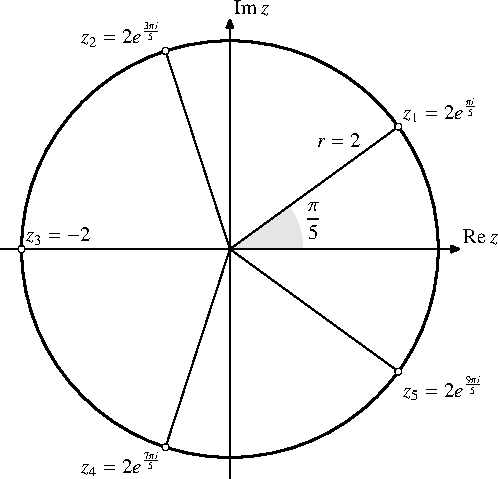
\includegraphics{uebungsaufgaben/exercise-1.pdf}
\caption{L"osungen der Gleichung $z^5+32=0$
\label{skript:15006:loesungen}}
\end{figure}
Wir suchen alle komplexen Zahlen in der Form $z=re^{i\varphi}$, es muss gelten
\begin{align*}
z^5&=r^5e^{5i\varphi}=-32
\\
r&=2\qquad\text{und}\qquad e^{5i\varphi}=-1
\\
\cos 5\varphi+i\sin 5\varphi&=-1
\\
\sin 5\varphi&=0
\\
\cos 5\varphi&=-1
\end{align*}
Die letzte Gleichung besagt, dass $5\varphi$ ein ungerades Vielfaches von
$\pi$ sein muss. Die zweitletzte Gleichung ist schw"acher, sie verlangt
nur, dass $5\varphi$ ein Vielfaches von $\pi$ sein muss, sie ist also
auf jeden Fall erf"ullt, wenn die letzte erf"ullt ist.
\[
5\varphi=(2k+1)\pi
\qquad\Rightarrow\qquad
\varphi=(2k+1)\frac{\pi}5
\]
$\varphi$ muss also ein ungerades Vielfaches von $\frac{\pi}5$ sein:
\[
\varphi\in\biggl\{
e^{i\varphi}\bigg|
\varphi
=
\frac{\pi}{5},
\frac{3\pi}{5},
\frac{5\pi}{5},
\frac{7\pi}{5},
\frac{9\pi}{5}
\biggr\}
\]
In der komplexen Ebene bilden die m"oglichen $\varphi$ ein regelm"assiges
F"unfeck (Abbildung~\ref{skript:15006:loesungen}).
Da das F"unfeck mit Zirkel und Linear konstruierbar ist, kann man
einen Wurzelausdruck f"ur Werte der trigonometrischen Funktionen 
finden, es gilt
\[
\cos\frac{\pi}{5}=\frac{1+\sqrt{5}}4
\qquad
\Rightarrow
\qquad
\sin\frac{\pi}5
=
\sqrt{1-\cos^2\frac{\pi}5}
=
\frac12\sqrt{\frac{5-\sqrt{5}}2}
\]
(siehe auch \cite{skript:pentagon}).
Daraus kann man jetzt auch die Winkelfunktionen f"ur die mehrfachen
Winkel berechnen:
\begin{align*}
\cos\frac{3\pi}5
&=
-\cos\frac{2\pi}5
=
-2\cos^2\frac{\pi}5+1
=
\frac{1-\sqrt{5}}4
\\
\sin\frac{3\pi}5
&=
\sin\frac{2\pi}5
=
2\sin\frac{\pi}5\cos\frac{\pi}5
=
\frac14\sqrt{10+2\sqrt{5}}
\end{align*}
Die "ubrigen Punkte des F"unfecks kann man durch Symmetriebetrachtungen
gewinnen.
Die gesuchten L"osungen sind also
\begin{align*}
z
\in
\biggl\{
&
\frac{1+\sqrt{5}}2+\frac{i}2\sqrt{10-2\sqrt{5}},\quad
\frac{1-\sqrt{5}}2 + \frac{i}2\sqrt{10+2\sqrt{5}},\quad
-2,
\\
&
\frac{1-\sqrt{5}}2 - \frac{i}2\sqrt{10+2\sqrt{5}},\quad
\frac{1+\sqrt{5}}2-\frac{i}2\sqrt{10-2\sqrt{5}}
\biggr\}.
\end{align*}
\end{loesung}


\end{uebungsaufgaben}

